\documentclass[12pt]{article}
\usepackage[margin=.8in]{geometry}
\usepackage{graphicx,hyperref,parskip}
\hypersetup{colorlinks,
    citecolor=black,
    filecolor=black,
    linkcolor=black,
    urlcolor=black
}

\newcommand{\HRule}{\rule{\linewidth}{0.5mm}}


\begin{document}
\newpage

\begin{titlepage}
\begin{center}
\textsc{\LARGE }\\[1.5cm]
\textsc{\Large Proposal 3}\\[0.5cm]

\HRule \\[0.4cm]
{\huge \bfseries Ripieno}\\
\HRule \\[1.5cm]

Tyler \textsc{Babaran}\\
Kevin \textsc{Carruthers}\\
Lara \textsc{Janecka}\\
Nik \textsc{Klassen}\\
Josh \textsc{Netterfield}\\
Eric \textsc{Pemberton}\\

\vfill
{\large \today}
\end{center}

Instructor: Christine Horton
\end{titlepage}

\tableofcontents
\newpage

\section{Ripieno}
\subsection{Introduction (Kevin)}
Ripieno is an upcoming music notation app brought to you by the Ripienist team.

Our team is developing Ripieno to fill a specific gap in the world of music notation: the missing ability to easily create and share sheet music. Any composer who wishes to share his work without Ripieno is forced to spend time scanning and compiling his written composition, transform that scan into a viewable file, and send that file to anyone who may be interested.

With Ripieno, all that composer would need to do is click the ``share'' button.

This product is useful for several reasons:
\begin{itemize}
\item teachers can use Ripieno to more easily teach their students; students can use Ripieno to learn about music composition
\item any composer, hobbyist or professional, can easily share their work
\item groups interested in composing a piece can work together
\end{itemize}

Ripieno is marketed towards local musicians, both hobbyists and professionals. In its simplest terms, Ripieno is of use to any individual with the desire to create or share sheet music; this can include music teachers, music enthusiasts, or even professional musicians.

More specifically, Ripieno is marketed towards Waterloo and Wilfred Laurier students: whether they are majoring in music or are simply interested in it, they can use Ripieno to explore their musical instincts.

For those students for whom music is a hobby, Ripieno can help them explore their interest without the hassle of dealing with multiple pieces of software, some of it difficult-to-use. Furthermore, hobbyist students do not need to worry about wasting their time finding a large variety of sources to help them compose---Ripieno will provide this for them.

For students majoring in music---either composition or performance---Ripieno provides essential tools comparable to the industry-leading software students use today. Instead of purchasing somewhere between two and six different tools to perform the various tasks necessary of any music student and still scrambling to share the work they do in each of those applications, students can find everything they need in one place: Ripieno.

\subsection{Proposed Project (Josh)}
Ripieno aims to make composing, sharing, and collaborating on sheet music easier for Waterloo and Laurier students.

To this end, Ripieno will be a high-quality, easy-to-use music scorewriter with an emphasis on collaboration and mobility. In particular, it is a web application as well as a native app for iPads, Macs, and PCs. Songs created on any platform are automatically synced to all other platforms and can be shared with any number of other users.

Professional sheet music notation software (``scorewriters'') currently on the market have a high barrier to entry both in terms of cost and usability, and sharing sheet music often involves printing it out due to incompatibilities in formats, even between versions of the same software. In addition, no professional sheet music engraver also provides mobile editing.

Students taking courses in composition and arranging can use the collaboration feature of Ripieno to submit assignments. Instructors can then make suggestions directly on the sheet music without printing. In addition, semi-professional musicians with a large library of music can use Ripieno to cheaply and efficiently manage and add to their repertoire.

\subsection{Costs and Requirements (Eric)}
The costs of developing this project are presented in three stages; product development, marketing and maintenance.

\begin{itemize}
\item {\bf Product Development}: The costs associated with developing Ripieno include the purchase of all required technologies to build the software, as well as the cost to hire software developers, UI designers and Quality Assurance personnel.
\item {\bf Marketing}: The costs for marketing the product will include online advertising, product demoes for interested parties, and brand promotion. Product demos will be scheduled for university professors and music students in high school and post-secondary music programs.
\item {\bf Maintenance}: Maintenance costs will include customer support, addressing bugs that clients discover, and developing fixes. In order to stay relevant in the industry software developers will develop new features based on user-feedback.
\end{itemize}

\subsection{Research (Nik)}
The age of digitization has affected almost every field, music included. Music stores are no longer able to maintain the market they once had due to the sheer amount of merchandise available online. The Joseph Patelson Music House in New York City is just one example of the many music stores that have closed due a lack of customers (Wakin, 2009).  Music students are now performing and composing their music using digital media. There are many tablet applications available to display music while performing. These applications allow users to download content from various music collections on the web (Rosen, 2011). However, changes to the way music is created are unable to proceed if composers do not have easy ways to create their sheet music digitally, leading to a need for Ripieno.

Composers working with publishing houses have access to proprietary software such as Finale, but with a price tag easily ranging beyond \$600, this software is inaccessible for educators and students (MakeMusic Software \& Accessories). Students are far less willing to take up a hobby if experimenting with it is expensive. In addition to cost, students wish to share their creative output with friends and get input from people with more experience.  According to students, a hobby or new field of study is much more fulfilling if they feel that they are making progress---and even more importantly, doing it properly. Our music notation app aims to make music easier to share, giving our users access to the collective knowledge of Ripieno community.

Schools and music software companies are already trying to get students involved in software creation.  Sibelius provides a feature for teachers to control copies of the software that their students are using in the classroom (Sibelius).  However, this doesn't allow students to collaborate with each other.  Another example of music notation software in education is Berklee Online's ``Music Notation Using Finale'' course, open to anyone (Feist, 2014).  This course aims to teach students how to use the software, but also fails to support student collaboration.

\subsection{Assets (Eric)}
To complete this project the following assets are available to the Ripieno team:
\begin{itemize}
\item The use of Javascript in the product is supported with extensive online documentation including design strategies for ``node.js''. This will cut down on the amount of time required to develop the product.
\item Music theory and notation is covered through a written notation book detailing every intricacy involved in rendering sheet music. This resource will allow Ripieno to create in-depth coverage of all music notation styles needed by users.
\item Musicians and music professors at the University of Waterloo are able to provide valuable input and feedback on how Ripieno can improve their courses and help their students.  This feedback will be useful in determining the features that are most important to our customers.
\end{itemize}

In using Javascript, we can ensure that product development is quick and easy. This will allow us to get our product in the hands of students as quickly as possible. Additionally, the extensive documentation will allow us to ensure our product is robust and works well.

The notation book and feedback from musicians will allow us to meet the needs of our customers by ensuring that whatever instrument they play, style of music they enjoy, or type of composition they favour, Ripieno will support it.

\subsection{Progress So Far (Kevin/Lara)}
\subsubsection{Accomplishments to Date}
After a few days of deliberation, the Ripienists had a detailed design plan outlined. Due to good group cohesion, a design was decided upon very quickly with full group consensus. Coming into the project, Josh already had a design in mind---thus accelerating the project development. There was a short discussion over which testing framework between Tyler and Eric during the third meeting which concluded in a method to ensure a bug free development evironment. The design planned was finalized after Nik and Josh finally agreed on the correct front-end framework to use. As a result of the first week of meetings the team has a design encompasing all aspects of the project including the barebones functionality of the applictaion and its tools, the layout of the user interface, and the methods of ensuring a bug free product. Overall, the team arrived an a collectively accepted and functional design to-be-implemented.

Currently, the team is just wrapping up the testing for a basic beta version of the final product. Rudimentary functionality has been achieved and testing has returned few bugs, all of which can bea easily fixed. Kevin has just finished some market research and is currently drafting changes to the user interface to make it more appealing to our potential clients.

\subsubsection{Future Goals}
Going forward, the Ripienists will be implementing the front-end interface changes as drafted by Kevin. Furthermore, there is a large list of features to be included in the next release:
\begin{itemize}
\item multi-staffed instruments
\item viewing multiple instrument lines simultaneously
\item collaborative chat
\item auto-import from tools such as Finale
\end{itemize}
and several others.

The features listed above will definitely be included in the next release, as well as fixes for any bugs our Quality Assurance team discovers in the meantime and any other features as time permits.

\begin{figure}[ht]
\centering
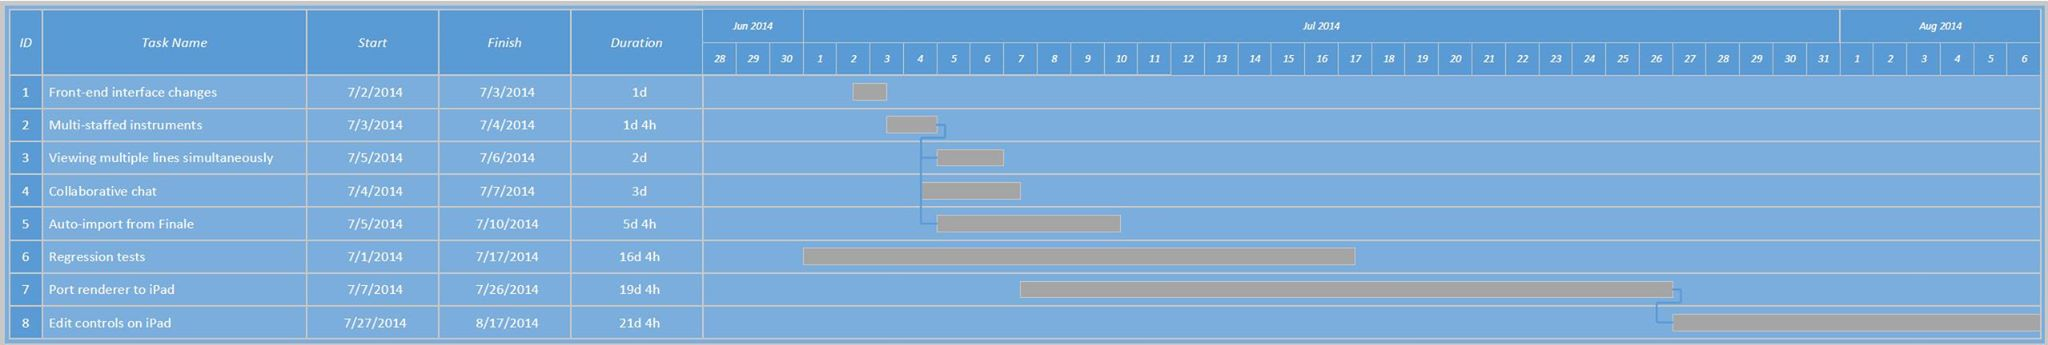
\includegraphics[width=\textwidth]{gannt.jpg}
\caption{Gannt Chart}
\end{figure}

\subsection{Team Structure (Tyler)}
The Ripienist team is structured as follows:
\begin{itemize}
\item Josh Netterfield is the creative genius behind Ripieno, and holds the final say on all creative descisions and the direction the project will be headed.
\item Nik Klassen is our assistant developer with four years of experience developing teaching tools at Desire2Learn. Together with Josh Netterfield, they are in charge of all coding, back-end development and user-interface design.
\item Lara Janecka will be operating as the project leader due to her experience in a managerial position at Auvik Networks Inc. She is responsible for ensuring the team meets deadlines, stays under budget, and maintains a positive work environment.
\item Kevin Carruthers has been designated chief of marketing. He is responsible for contacting new investors, creating advertisements, and ensuring that the world knows about Ripieno and all it can provide.
\item Eric Pemberton and Tyler Babaran are specialists in Software Quality Assurance and testing. They are responsible for ensuring that all aspects of Ripieno are working as expected upon release.
\end{itemize}

\subsection{Conclusion (Lara)}
Ripieno fills a much needed niche in Waterloo. The music departments within the University of Waterloo and Wilfred Laurier University provide a large market of young musicians who are already share large portions of their lives via the Internet and currrently lack an affordable and convenient way to do so. Musicians are often very passionate toward their craft and need a way to easily share this with others. Ripieno allows musicians to share and collaborate with the same ease as one might share a project proposal via Google Docs. Based on the above results, the Ripienist team would like to proceed with the development of the project.
\newpage

\section{Sources}
\begin{enumerate}
\item Wakin, D.  (2009).  Swan Song for a Music Store and Clubhouse.  \emph{New York Times}.  Retreived from http://www.nytimes.com/2009/04/13/arts/music/13pate.html?\_r=0
\item Rosen, R.  (2011).  Musicians Embrace the iPad, Leave Sheet Music at Home.  \emph{The Atlantic}.  Retrieved from http://www.theatlantic.com/technology/archive/2011/08/musicians-embrace-the-ipad-leave-sheet-music-at-home/243726/
\item MakeMusic Software.  Retreived from https://store.makemusic.com/Store/default.aspx?tab=notation
\item Sibelius.  Retrieved from http://www.sibelius.com/products/sibeliusedu/7/index.html
\item Feist, J.  (2014).  Music Notation Using Finale.  \emph{Berklee Online}.  Retrieved from http://online.berklee.edu/courses/music-notation-using-finale
\end{enumerate}

\end{document}
